\section{Explicit polynomial instances and executable evidence}
\label{sec:examples}

\subsection{The upper branch of the unit circle}

Take
\[
 F(x,y)=x^2+y^2-1,\quad (a,b)=(0,1),\quad
 A=\tfrac12,\quad H=\tfrac12F,
\]
and
\[
 |x|\le\tfrac14,\qquad |y-1|\le\tfrac14,\qquad
 r=\alpha=\tfrac14,\quad M=\tfrac14.
\]
Then \(U=x\), \(V=y\), and
\[
 |1-V|\le\tfrac14\le\tfrac12,\quad |U|\le\tfrac14,\quad
 H(0,1)=0,\quad M\alpha=\tfrac1{16}=r/4.
\]
The evaluator and Jacobian evaluator are exact rational
polynomials. With \(d=\max(|h|,|k|)\),
\[
 H(x+h,y+k)-H(x,y)-xh-yk=\tfrac12(h^2+k^2),
\]
whose absolute value is at most \(d^2\).
Also the full row norm of the Jacobian difference is
\(|h|+|k|\le2d\). Thus raw moduli
\[
 \mu_0(p)=p,\qquad \nu_0(p)=p+1
\]
satisfy R3--R4; R0--R2 follow from the displayed polynomial
identities and box bounds.

The resulting branch is characterized by
\[
 x^2+g(x)^2=1,\quad \tfrac34\le g(x)\le\tfrac54,\quad
 g(0)=1,\qquad g'(x)=-\frac{x}{g(x)}.
\]
It is the positive square-root branch; that description
is a consequence of the constructed zero and uniqueness,
not an input square-root oracle.
The general estimates give
\[
 |g(x)-g(x')|\le\tfrac12|x-x'|,\qquad
 \mu_g(p)=p+3,\quad \nu_g(p)=p+5.
\]
Here \(s=0\), so precision \(k\) uses exactly \(k+4\)
steps at evaluation and rounding precision \(k+5\).

\begin{figure}[htbp]
 \centering
 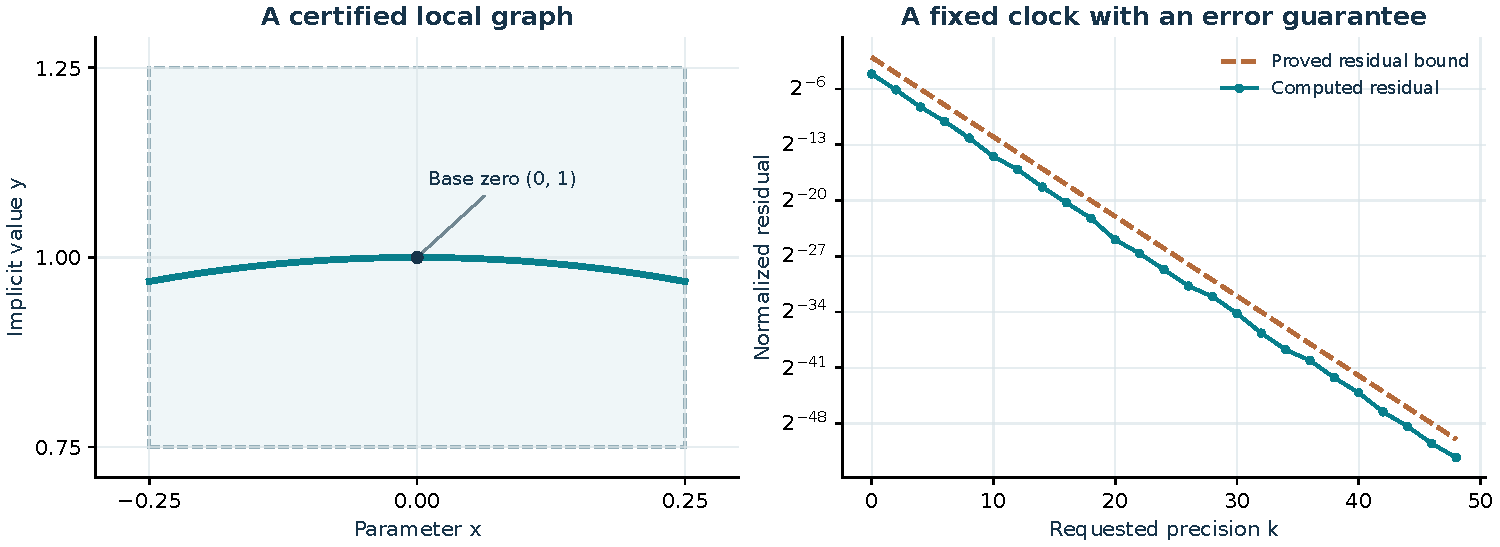
\includegraphics[width=\textwidth]{figures/implicit_graph.pdf}
 \caption{The circle example. Left: the certified rational box
 and the unique upper branch on the parameter interval.
 Right: exact-rational residuals from the implemented finite
 program, displayed on a logarithmic scale, together with the
 proved bound \(2^{-(k+2)}\). Floating-point conversion is used
 only to draw this figure; the validation inequalities use
 exact fractions.}
 \label{fig:circle}
\end{figure}

\subsection{A coupled two-dimensional vertical system}

To exhibit a matrix-valued vertical derivative, set
\[
 H(x,y_1,y_2)=
 \begin{pmatrix}
  y_1+\tfrac14y_1y_2-x\\
  y_2+\tfrac14y_1^2-\tfrac12x
 \end{pmatrix},
 \quad |x|\le\tfrac1{16},\quad |y_1|,|y_2|\le\tfrac14.
\]
The center is zero, \(A=\Id\), \(r=1/4\), \(M=1\), and
\[
 U=\begin{pmatrix}-1\\-1/2\end{pmatrix},\qquad
 V=\begin{pmatrix}
  1+y_2/4&y_1/4\\
  y_1/2&1
 \end{pmatrix}.
\]
Each row of \(\Id-V\) has absolute row sum at most \(1/8\).
The parameter condition is \(M\alpha=1/16=r/4\).
The Taylor remainders are \(k_1k_2/4\) and \(k_1^2/4\),
so their maximum is at most \(d^2/4\).
The full Jacobian changes by at most \(d/2\).
One may therefore take \(\mu_0(p)=\nu_0(p)=p\).
All raw certificates are rational polynomial inequalities.

The theorem gives a unique vector branch
\((g_1(x),g_2(x))\), Lipschitz constant \(2\), and the
explicit derivative equation
\[
 \begin{pmatrix}
  1+g_2/4&g_1/4\\
  g_1/2&1
 \end{pmatrix}
 \begin{pmatrix}g_1'\\g_2'\end{pmatrix}
 =\begin{pmatrix}1\\1/2\end{pmatrix}.
\]
The generic moduli are \(\mu_g(p)=p+5\) and
\(\nu_g(p)=p+6\).
The rational Neumann program computes this derivative
without needing a symbolic inverse formula.

\subsection{A simple nonlinear inverse with all assumptions discharged}

For an additional compact arithmetic instance, take
\[
 H(x,y)=y+y^3-x,\qquad
 |x|\le\tfrac1{16},\quad |y|\le\tfrac14.
\]
Here \(U=-1\), \(V=1+3y^2\), \(M=1\), and
\(|1-V|\le3/16\). The Taylor identity is
\[
 H(x+h,y+k)-H(x,y)+h-(1+3y^2)k=3yk^2+k^3.
\]
Because both vertical endpoints lie in the box,
\(|k|\le1/2\), and the remainder is at most
\((3/4+1/2)d^2\le2d^2\).
The derivative change is bounded by
\(3|y-y'||y+y'|\le(3/2)d\le2d\).
Thus \(\mu_0(p)=\nu_0(p)=p+1\) suffices.
The theorem constructs the unique local solution of
\[
 g(x)+g(x)^3=x,\qquad
 g'(x)=\frac1{1+3g(x)^2}.
\]
This instance needs only rational polynomial identities
and elementary order bounds; no pre-existing theorem
about cubic roots, implicit functions, or real completeness
is needed to discharge its input contracts.

\subsection{What the code verifies}

The executable implementation uses Python integers and
\code{fractions.Fraction}; it requires no third-party
packages. It implements \eqref{eq:algorithm} exactly and
uses explicitly bounded loops. The validation file contains
the deterministic results and hashes of the source files.

The supplied validation completed \(4{,}680\) traces:
two polynomial providers, nine parameter points per
provider, every requested precision from \(0\) through
\(64\), and four oracle modes. The additional modes add
controlled positive, negative, or varying errors of
size at most the allowed evaluation error.
The checks include \(168{,}480\) individual steps and
\(2{,}048\) aligned trace comparisons.

In total, \(1{,}317{,}978\) exact-rational assertions passed.
They check domain preservation, evaluation and rounding
budgets, the scaled recurrence invariant, the terminal
residual bound, parameter sensitivity, finite Neumann
identities, and derivative calculations against an
independent rational matrix inverse. Special cases exercise
negative dyadic flooring and clipping at both endpoints
of a non-dyadic interval. The circle example also has
independent exact polynomial root brackets.

These computations establish that the implementation and
the displayed constants agree on the tested cases.
They do not establish the universally quantified raw
certificates by sampling, and they are not an iPRA proof
checker. The mathematical proofs of the certificates
and general theorem are the algebraic arguments above;
the separate Lean core checks specific finite lemmas.
